\documentclass[a4paper,11pt]{article}


\usepackage{amsmath,amsfonts,amsthm,a4wide}
\usepackage{graphicx}
\usepackage[super]{nth}
\usepackage{mathtools}


\begin{document}
\begin{center}
University of Toronto at Scarborough\\[0.1in]
{\bf CSCC73H3 Algorithm Design and Analysis, FALL 2018} \\[0.1in]
{\large{\bf Assignment No.7: Linear Programming }}\\[0.1in]
{\bf DUE:} November 24, 2018, at 11:59 pm
\end{center}


\vspace{0.1in}
\noindent
{\bf Student ID:} 1005642654 \\[0.15in]
{\bf Student Name:} KyooSik Lee
\vspace{0.3in}

\vspace{0.3in}
\begin{enumerate}

\item 

\begin{enumerate}
\item
Let's say the number of package A that the company decides to make is $x$, and the number of package B $y$. Then the objective function is the profit. The total dried fruits is $x+2y$ $lb$ and the total nuts is $1.5x + y$ $lb$. So buying the bulk is total $4x+4y$ dollars. Also, packaging is $1.4x + 0.6y$ dollars. The money by selling is $7x + 6y$ dollars. So the profit is $(7x + 6y)-(4x + 4y)-(1.4x+0.6y)$. Therefore the objective function is $1.6x + 1.4y$.

Now the constraints.

Because factory can only produce 110000 of A, $x\leq 110000$.

Because there are total 240000 $lb$ of dried fruts and 180000$lb$ of nuts, $x+2y \leq 240000$ and $1.5x+y \leq 180000$.

And because there should be at least one package for A and B, $x \geq 0$ and $y \geq 0$.

\item
Following is the plotted graph.
\begin{figure}[hbt]
	\centering
	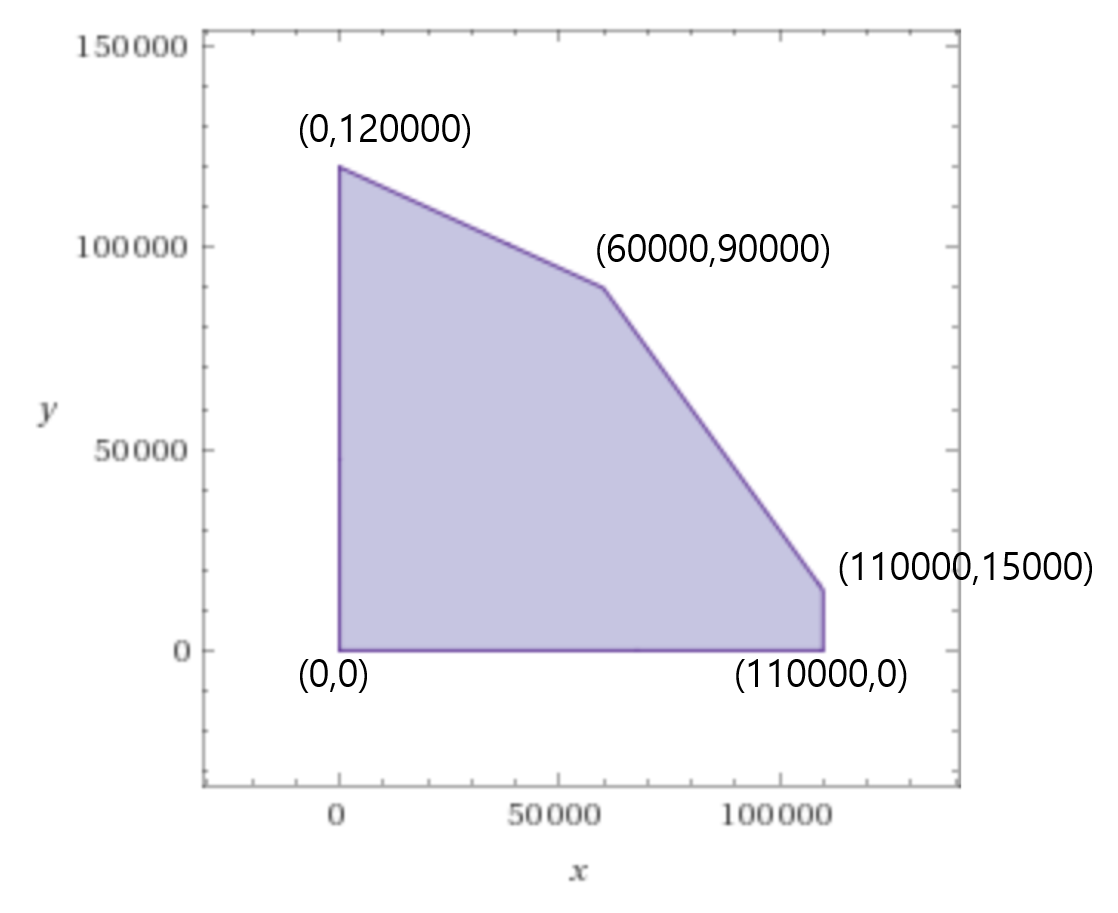
\includegraphics[scale=0.4]{figure1.png}
	\caption{Feasible Reigion}
\end{figure}

The vertex maximizing the profit is $(60000,90000)$.

\item

Let's use the simplex method.

The objective function is $1.6x + 1.4y$. and the constraints are $x \leq 110000$, $x+2y \leq 240000$, $1.5x+y \leq 180000$, $x \geq 0$, $y \geq 0$. Let's label each constraints $c_i$. (i = 1, 2, 3, 4, 5)

Then increase y to make $c_3$ tight. so $y = 120000$. And lets shift to make a new origin. Let $x_1 = x$ and $y_1 = 240000 - x - 2y$. Then we have our constraints with $x_1$ and $y_1$. $c_2 $ is tight, $c_5$ is released.

The new constraints are $x_1 \leq 110000, y_1 \geq 0, x_1 - 0.5 y_1 \leq 60000, x_1 \geq 0, x_1 + y_1 \leq 240000$. And the new objective function is $0.9x_1 - 0.7y_1 + 168000$. Now $x_1$ has positive coefficient, so increasing $x_1$ increases the objective function.

Then $c_4$ is released, $c_3$ is tight. So let $x_2 = 60000-x_1+0.5y_1$, $y_2 = y_1$. So the new constraints are $-x_2 + 0.5y_2  \leq 50000, y_2 \geq 0, x_2 \geq 0, x_2 - 0.5y_2 \leq 60000, x_2 - 1.5y_2 \geq -180000$. And the objective function is $222000 - 0.25y_2-0.9x_2$. The coefficients are all negative, and this is the optimal point. The optimal value is 222000.
\end{enumerate}


\item 
All the value $|ax_i + by_i - c|$ must be bounded by the maximum value,$\max_{1\leq i\leq 7} |ax_i + by_i - c|$. Finding the minimum value of this maximum value is to make a new variable $k$, which will be the maximum value.

Then the objective function is $k$. We will try to minimize this.

Because every $|ax_i +by_i - c|$ is bounded by $k$. The constraints are the following.

$|10a +19b-c|\leq k$

$|8a +15b-c|\leq k$

$|7a +14b-c|\leq k$

$|5a +11b-c|\leq k$

$|3a +7b-c|\leq k$

$|2a +5b-c|\leq k$

$|1a +3b-c|\leq k$

But this is not linear, so making the constraints to follow linear programming, the real constraints are following.

$10a +19b-c\leq k$

$10a +19b-c\geq -k$

$8a +15b-c\leq k$

$8a +15b-c\geq -k$

$7a +14b-c\leq k$

$7a +14b-c\geq -k$

$5a +11b-c\leq k$

$5a +11b-c\geq -k$

$3a +7b-c\leq k$

$3a +7b-c\geq -k$

$2a +5b-c\leq k$

$2a +5b-c\geq -k$

$a +3b-c\leq k$

$a +3b-c\geq -k$

\end{enumerate}



\end{document}

\iffalse
\begin{figure}[hbt]
	\centering
	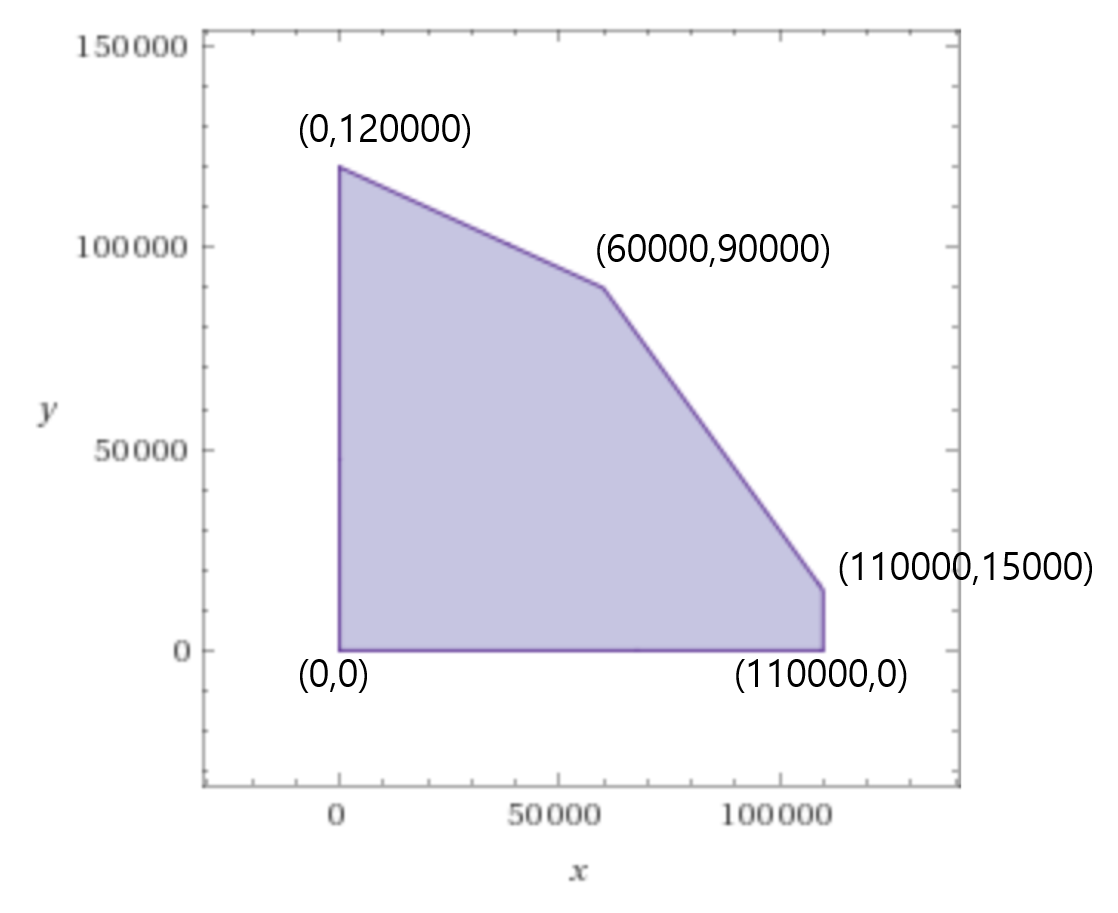
\includegraphics[scale=0.4]{figure1.png}
	\caption{Basic Tree}
\end{figure}
\fi
